\chapter{引言}
\label{chap00}
语义Web(Semantic Web)是Web(万维网)的一个重要发展方向,它提供一个通用框架,
使得数据的共享和重用可以跨越应用系统、企业和社区的边界。在原始Web上只有文档的
交换和共享,语义Web以RDF(Resource Description Framework)为基础,而RDF以URI
(Uniform Resource Identifier)作为标识机制、XML作为语法,能够将各种不同应用中
的数据和服务容易地集成起来。本体(ontology)在语义Web中扮演着重要的角色,语义
Web本体一般是指使用RDFS(RDF Schema)或者OWL(Web Ontology Language)等语言描述
的本体,其中定义了类(class)、属性(property)和实例(instance)。而类、属性和
实例又可统称为实体(entity)。近年来,有关RDF数据查询的SPARQL和有关规则表示的
RIF(Rule Interchange Format)等技术也日趋成熟,标志着语义Web的数据模型、本体
语言、规则语言和数据存储等技术基础已经奠定。

随着语义网(Semantic Web)的快速发展,语义网数据大幅增长。本体(ontology)作为
语义网的基础,它是领域知识概念化和模型化的一种重要途径,被用来描述数据的
语义信息。迄今为止,语义网搜索引擎Falcons\cite{1}已经采集到超过2.5万个语义网本
体。尽管语义网技术在生命科学等领域已经取得了阶段性成功,但是它距离广泛应用仍有
很长一段距离,其中一个主要的原因是由于当前万维网上绝大多数的数据是以关系数据库
的方式存储(约占77.3\%,俗称``deep Web''\cite{2}),导致语义网应用不能自由地访
问和操纵这些数据,从而限制了语义网的发展。万维网的发明人和语义网的倡导者Tim
Berners-Lee先生也撰文指出,世界上的很多数据仍然封闭在数据库中,尚未在万维网上
以资源的形式公开发布\cite{3}。

关系数据库和本体的数据互操作性问题,一部分可归结为关系数据库模式和本体间的映射
问题\cite{4}。传统关系数据库中,关系表的结构及其完整性约束都由关系数据库
模式定义,并且关系数据库模式和本体间存在着许多近似的对应关系。例如关系数据库
模式中的列可以对应到本体中的属性。事实上,关系数据库中的许多原语都属于一阶逻辑
范畴\cite{5},而最常见的OWL DL本体\cite{6}的逻辑基础为描述逻辑语言
$\mathcal{SHOIN(D)}$,描述逻辑是一阶逻辑的一个子集。因此,建立关系数据库模式和
本体间的映射在理论上是可行的。

现实世界中,不同的关系数据库通常拥有不同的数据模式,而万维网和语义网的分布性
使得不同领域乃至相同领域的不同组织也可能定义不同的本体,这造成了现实中存在众多
异构的关系数据库模式和本体。由于数量、规模等原因,通过人工方式发现关系数据库模式
和本体间的映射非常耗时耗力。国内外研究人员已经提出了一些(半)自动化的关系数据
库模式和本体间的映射方法\cite{4,7}。这些方法大致可分为两类:一类是发现关系数据
库模式中元素(表、列)和本体中元素(类、属性)之间一对一的简单映射;另一类是基于
简单映射生成多对多的复杂映射。

本文提出一种基于语义的关系数据库模式和本体间的映射方法SMap,既能够发现元素之间的
简单映射也能学习复杂映射,具体流程见图\ref{fig:0}。SMap首先采用逆向工程规则,启
发式地将关系数据库模式和本体中的元素对应地划分到4个不同类别中,再针对不同类别中
的元素引入不同的相邻元素的自然语言描述来构建虚拟文档,通过计算虚拟文档间的相似
度来发现元素之间的简单映射。接下来,基于这些简单映射以及重叠的实例数据(数据库
记录、本体实例)生成训练事实集合,采用一种自底向上的归纳逻辑编程算法GOLEM
\cite{8}学习出元素之间的3种复杂映射。这些以Horn规则形式表达的复杂映射可以很容易
地转换为条件查询。在6组真实数据集上的实验结果表明,SMap无论是在简单映射发现还是
在复杂映射学习上均明显优于5个现有的关系数据库模式和本体间的映射方法。

\begin{figure}[htdp]
\centerline{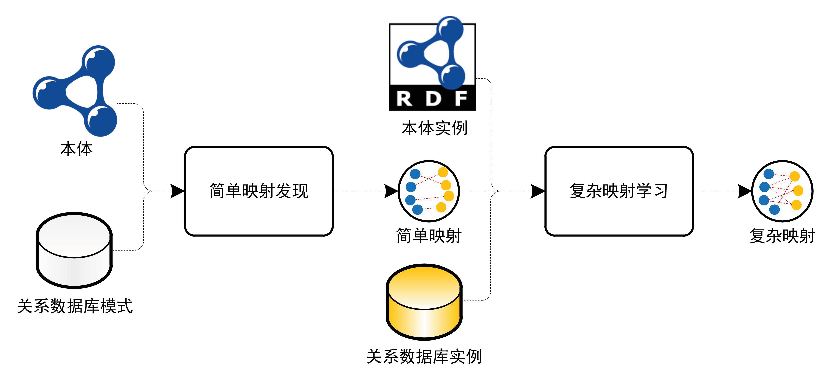
\includegraphics{0.eps}}
\caption{关系数据库模式和本体间语义映射发现流程}
\label{fig:0}
\end{figure}

文章的组织结构如下:第\ref{chap01}章介绍相关工作并给出问题定义;第\ref{chap02}、
\ref{chap03}章分别介绍简单映射的发现方法和复杂映射的学习方法;第\ref{chap04}章
介绍原型系统的设计实现并测试方法的有效性;最后总结全文。
